\documentclass[a4paper, openany]{memoir}

\usepackage[utf8]{inputenc}
\usepackage[T1]{fontenc} 
\usepackage[english]{babel}
\usepackage{amsmath}
\usepackage{amssymb}

\usepackage{booktabs}
\usepackage{fancyhdr}
\usepackage{float}
\usepackage{indentfirst}
\usepackage{graphicx}
\usepackage[linewidth=1pt]{mdframed}
\usepackage{multicol}
\usepackage{fancyvrb}

\pagestyle{fancy}
\fancyhf{}
\fancyhead[LE]{\leftmark}
\fancyhead[RO]{\rightmark}
\fancyhead[RE, LO]{PSD}
\fancyfoot[LE, RO]{\thepage}
\fancyfoot[RE, LO]{Pete Gautam}

\renewcommand{\headrulewidth}{1.5pt}

\chapterstyle{thatcher}
\setcounter{chapter}{12}

\begin{document}
\chapter{Systems scale testing}
Non-functional requirements describe emergent characteristics and properties of an overall system. These must be measured to be satisfied rather than being observed as a provided feature, which was possible for functional requirements. For this reason, non-functional requirements cannot typically be checked for in unit tests or through static analysis. They can only be tested once the implementation of the system has been realised.

The implementation tested may be the final system or a prototype. It may also be possible to build a model from which the characteristics of the final system can be approximated. Non-functional requirements may act as an aggregate for a set of more complex and interacting functional properties that are too difficult to test individually.

Conducting a test for non-functional requirements is similar to a scientific experiment. The tester forms a hypothesis for the system under test, based on the requirements. Then, they conduct an experiment to determine whether the hypothesis is satisfied. A well-formulated non-functional requirement should describe:
\begin{itemize}
    \item the property of the system to be measured. This is the abstract property that should be described by a well-formulated non-functional requirement.
    \item the metric to be used. This is the concrete property.
    \item the operating conditions in which the requirement must be satisfied.
    \item the threshold the system behaviour must exceed to satisfy the requirement.
\end{itemize}

There are many categories of non-functional requirements. Each category can be tested in several ways. We will provide a high-level outline of some of the categories.

\section{Safety-critical environments}
The operation of a particular system might occur in conditions that are particular harmful to the system (or the humans) that depend on the system. This may be because of adverse environments in which the system operates, or the nature of the system itself if it were to malfunction. Examples of such softwares are: 
\begin{itemize}
    \item automatic pilots for transportation, such as in aeroplanes;
    \item equipment used in the operation of particle beam radio-therapy equipment;
    \item space-based technology, such as satellites, space craft and planetary rovers;
    \item nuclear power station management systems.
\end{itemize}

These systems are called safety-critical system. A principal concern for the system design and evaluation process is to gain confidence that the operation of the system will not cause the system or its users any harm. 

If we have a system that controls a safety-critical system's behaviour, then we need to be sure that the other system too is safe. Testing safety of the system is concerned with developing test cases which demonstrate that the harm will not be caused on the adverse environment in which the system will be used.

\section{Reliability testing}
Reliability is the extent to which a system performs according to its specification. It can be measured by the following metrics:
\begin{itemize}
    \item the probability of failure on demand. This provides an estimate of the probability of failure each time a system is accessed.
    \item the mean time to failure. This indicates how long it takes for a software system to fail from initiation, or the average time between failures. It is a useful metric for systems where it is difficult or expensive to access them for repairs, such as a space level systems. We want the mean time to failure should be greater than the mission time.
    \item the down time, e.g. per year. This indicates how much time can be lost on system outages over a period of time. It is useful for high demand continuous use systems, such as high-volume transaction processing or commercial systems. For instance, payment systems are often designed to have downtime of less than a few seconds a year.
\end{itemize}

There are several methods for testing systems safety:
\begin{itemize}
    \item Model driven development allows for the implementation of the software test suites to be generated automatically from platform-independent models. The test cases are derived from assertions about the legal and the illegal states for the software model.
    \item Clean room development uses automated and statistical methods to select test cases for execution. It is used to calculate an estimate for the software system's probability of failure on demand, and a confidence in the estimate.
    \item Hazards and Operability Analysis (HAZOPS) is derived from chemical engineering. For a software, HAZOPS-like process caan be used to identify flows of information (instead of chemicals) between software components. We can then ask
    \begin{itemize}
        \item how the flows of information between software components are made.
        \item what will happen in different circumstances (e.g. if the information is incorrect or if it arrives too early/late).
    \end{itemize}
\end{itemize}

Emphasis in use of formal methods for tests allows us to gain accurate measurements about the reliability of the system. It also provides inputs into a safety case. Safety cases are justifications that a system meets its safety requirements. 

On the other hand, HAZOPS looks at the consequences of failures of one or more system components, or when they do not perform as expected. It is used to gain assurance of the reliability and the safety of the system in the presence of a failure.

\section{Hostile environments and security testing}
A hostile environment is one where we assume that there is an active agent. These can be threats or attackers. Their goal is to deliberately penetrate, subvert or sabotage a deployed system. Examples include:
\begin{itemize}
    \item Electronic voting systems, which are threatened by agents who want to subvert the results.
    \item Automatic teller machines, which are threatened by those who want to get access to administrative user interfaces (e.g. ATM) to steal money.
    \item Friend-or-foe detecting systems, which are threatened by enemies who want to trick those in firing on friendly aircrafts, for example.
    \item Digital rights management systems, which are threatened by copyright pirates who want to make unauthorised copies of the digital media for resale.
    \item Network security systems (such as firewalls), which are threatened by attackers who wish to gain unauthorised access to vulnerable servers.
    \item Authentication systems, which are threatened by attackers who wish to gain unauthorised access to information.
    \item Digital cash.
\end{itemize}

Disturbed systems in particular (or their components) are often considered to operate on a hostile environment because some (or all) of the network's participants are not known to the system itself.

System threats actively search for defects in the system that could be attacked. So, it is necessary to conduct tests to gain assurance that the system is resistant to these sorts of attacks. Security testing metrics include:
\begin{itemize}
    \item attacker capabilities or the knowledge required to penetrate the system.
    \item time and resources to penetration, i.e. we estimate how long it will take for an adversary/attacker and how much resources are required to penetrate the system.
    \item unpatched vulnerabilities per line of code.
    \item patched issues per year.
    \item successful penetrations per year.
    \item attack surface exposure.
\end{itemize}

\section{Security testing methods}
A number of security testing methods are also possible, including vulnerability testing such as
\begin{itemize}
    \item SQL injection testing,
    \item port scanning, and
    \item fuzz testing.
\end{itemize}
In fuzz testing, a software system is applied with unusual and malformed (i.e. fuzzed) inputs that may cause the system to behave in an unexpected/insecure way. It is a way of checking the extent to which the inputs are validated before they are passed on to business logic code. For example, it is an effective means of detecting buffer overflow vulnerabilities.

Penetration testing is a method in which the attack (red) team is tasked with gaining unauthorised access to the resources protected by the system. These are assumed to have the same resources as the attacker. The process may concentrate on technical vulnerabilities or engage in social engineering to gain access to the system.

\section{Performance testing}
Performance testing is how a system copes with different rates of input. There are several properties of interest, such as:
\begin{itemize}
    \item throughput, which is the amount of transactions that a system can process in a fixed amount of time.
    \item demand, which is the maximum rate of transactions that a system can process concurrently.
    \item response time, which is the maximum length of time taken to respond to an individual transaction request.
\end{itemize}

Once a property metric has been selected, there are 2 types of tests we can perform with respect to the threshold:
\begin{itemize}
    \item a limit test, which demonstrates that the system behaves normally within a required limit. This is typically used to demonstrate that a system behaves as expected within a required operation limit.
    \item a stress test, which discovers what happens when a particular limit is breached. This is used to discover how a system behaves beyond the operation limit specified. It is typically used to demonstrate that a system continues to behave reliably and predictably when operating outside of the normal limit. For example, the system's response to excessive demand may be to revert to a safe mode. This might only offer a limited service to the clients. Alternatively, it may be required that the system performs a graceful and safe shutdown rather than fail completely. For example, database servers are often equipped with uninterruptible power supplies (UPS). If there is a power loss, the battery power is used while the server completes any outstanding transaction on the database and then initiates a clean system shutdown.
\end{itemize}

\section{Scaling effects in systems testing}
In acceptance testing, we saw 3 types of testing- unit testing, integration testing and system testing. We can evaluate a test case in terms of its effectiveness and efficiency. The issue with systems testing is that as the size of the software system increases, the number of tests required for a given level of effectiveness increases exponentially. This is because the number of possible paths through the program or the states the program can be in increases exponentially as the size of the system increases linearly. We can see this in the figure below.
\begin{figure}[H]
    \centering
    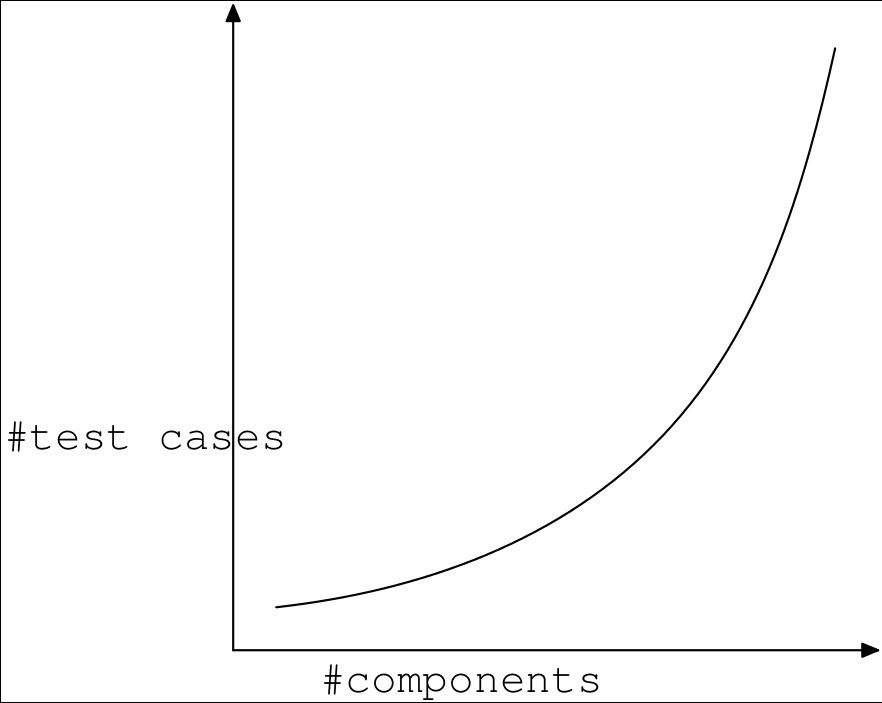
\includegraphics[scale=0.3]{src/13 components v test cases.png}
\end{figure}
\noindent This has a knock-on effect impact on efficiency. As the level of effectiveness increases, the cost of maintaining the test suite increases exponentially. So, there is an exponential decline in efficiency as the system grows.

\section{Dimensions of scale}
Scale can affect different characteristics of the software system. It has different impacts on testing. There are different measurements of scale, such as:
\begin{itemize}
    \item the number of lines of code,
    \item the number of software modules and inter-dependencies,
    \item the number of software platforms,
    \item the variations in build and configuration of deployments,
    \item the duration and variation in inputs that a system might experience,
    \item the software development team size, location and experience,
    \item the number of geographical locations and network connections, and
    \item the number and variation in users.
\end{itemize}

Performing system tests at the right scale can be very expensive if not infeasible, no matter which metric we choose. The development team needs to develop a system test suite that carefully prioritises the most important properties, features or the use cases of a system.

\section{Heterogeneous systems}
Large-scale software development efforts, with hundreds of thousands or millions of lines of code are often divided into one or more teams of developers. Each team is given the responsibility for development, testing and delivery of one or more of the subsystems. Such heterogeneous software projects may be composed of:
\begin{itemize}
    \item different business units within a single organisation,
    \item business units form different subsidiaries within the same umbrella organisation,
    \item project teams with different organisations brought together as part of a constorium,
    \item many individuals from different organisations.
\end{itemize}
The greater the variation in the organisational culture (i.e. the different outlooks, social backgrounds, management styles between the teams), the harder it can be to develop a consistent test program for the software project. Each organisation will have its own workflow for development and quality assurance. 

Even though there might be agreed standards, natural variation will occur. It becomes harder to achieve consistent and coherent software quality for the overall system. Also, being overly restrictive might reduce the productivity of the team, create tension or conflict between competing standards or ways of implementing standards. This could delay integrations as the teams are reluctant to be challenged and can deter participance from being collaborators.

Free and open source projects are good examples of this. Such projects must achieve a balance between attracting new contributors and maintaining sufficient quality and standards within the codebase.

An example of a heterogeneous system is the ATLAS project. It is a project supported by a large-scale software project. In particular, there are:
\begin{itemize}
    \item 7 million source lines of code,
    \item 10 major subprojects,
    \item multiple platforms, compilers, languages and configurations, and
    \item 500 developers,
    \item 3000 users (scientists and engineers), and
    \item 40 countries.
\end{itemize}

The project team has developed an extensive build test infrastructure to manage the collaborative software effort. They cannot run all tests on every commit since it is be infeasible. Rather, the core engineering team have developed a suite of tests that run periodically to provide a health status for the software project, including:
\begin{itemize}
    \item ATLAS testing nightly,
    \item ATLAS run time tester,
    \item ATLAS nightly build,
    \item Full chain test,
    \item Tier0 chain test,
    \item Big chain test, and
    \item SampleA test.
\end{itemize}

\section{Socio-technical systems}
Socio-technical systems (also called computer-based systems) incorporate both computer software and hardware, the computer system users and surrounding organisation and cultural practices. The system boundary is drawn around the organisation as a whole. So, the software and the hardware systems are just some of the components to be considered in the overall system to be tested. 

This perspective introduces socio-technical issues of scale and complexity. From this perspective, the organisation as a whole must be tested when a new software system is introduced, and not just the software itself. Introducing a new software system will cause the rest of the organisation to evolve in response. We need to test the whole system for potential defects which have been introduced by the evolution.

Testing socio-technical systems effectively is challenging because:
\begin{itemize}
    \item the members of the organisation may be working and therefore unavailable to take part in the tests.
    \item obtaining realistic test scenarios may not be practical. It may not be perceivable what the scenarios may be.
    \item identifying and covering the real working practices may prove difficult. Managers often have a very good understanding of the idealised view of what a workflow is in the organisation. But, the individual workers may adapt and evolve this practice in order to optimise their own workflow in complex ways and to deal with contingencies.
    \item the organisation may evolve independently of the system as new business challenges and requirements arise.
\end{itemize}

For example, assume that a student management system is being designed for a university. The system is likely to be procured and developed to replace an older one. So, while the new software is being developed, the old system is in constant use. Running system tests with sufficient number of users (employees and students) doing all the strange and unusual things to put the system under sufficient stress will be difficult since they will not be constantly available (and not all of them). 

The actual workflow around the old system may be poorly understood. The managers will have an abstracted understanding of how the system should be used. But, in practice, different academic units within the university will have developed specialised local workflows to suit their needs. Moreover, actual users will have developed much more complex workflows to handle for a wider range of contingency and exceptions than the managers and the software developers are aware of. These scenarios are not likely to be represented in system tests.

The procurement process for the new system may last several years. The university might have changed considerably over this time, perhaps due to administrative reorganisation. So, the new information system may not integrate well to its new environment for this reason.

Another example of socio-technical issue is the 2007 Scottish election counting system. The development team invested significant resources in testing. They paid for hundreds of thousands of ballot papers to be manually completed for each deployment of the system so that the acceptance testing process could be completed before the election night. 

However, the system still experienced significant problems during the night. The system needed to be able to process hundreds of thousands of ballots, not tens of thousands. It struggled with this workload. The workers using the system became increasingly familiar with it overnight. They began to optimise their workflows in unexpected ways. There were a variety of ways a ballot paper was completed by the voters, and not all of these were anticipated. In fact, there was a higher spoilt/rejected ballot rate than was expected. This caused the indexed databases (where the results were being stored) to be corrupted. Overall, the case study does not show that the resources allocated to testing, but only shows the difficulty of doing so.

\section{System of systems}
Sometimes called joint systems or a coalition of systems, a system of systems represents the extreme end of scale for challenges in software testing. A system of systems represents multiple heterogeneous semi-autonomous systems that cooperate and coordinate to produce emergent effects, e.g. electronic stock exchanges, military coordinate systems across multiple arms of the military or different militaries, air traffic control systems and supply chain control systems.

A system of systems is not under the control of any real coordination of any one actor. Individual systems may evolve independently of neighbouring systems and overall the system of systems itself. So, testing such a system is extremely challenging. In particular:
\begin{itemize}
    \item Each member system has its own cultures and practices.
    \item The system cannot be isolated or configured for a test.
    \item One of the member systems may evolve during a test.
    \item The expected outputs for a system are not easy to define.
\end{itemize}

An example of this is the flash crash in May 2010. This caused a rapid collapse and recovery in the stock prices over about half an hour. Modern stock markets are extremely complex. They are controlled by a diverse range of trading applications and algorithms, all developed and maintained as proprietary software by a wide range of financial institutions.

Understanding the interplay between rapidly evolving software systems and their users is extremely difficult. This makes testing the overall stock market for resilience quite difficult.

\section{Getting feedback from the wild}
Due to the difficulty of running acceptance tests, many development teams have augmented their applications with mechanisms for gathering information from the users directly. It can be automated submissions of crash reports, including stack traces and heap states. It can also be facilities for manually submitting defect reports within application.

The approach turns user system into its tester. It leverages scaling effects to mitigate problems of large scale system testing. But, this need not work in practice. This approach is dependent on having users who are willing to cooperate as often, unpaid testers. Mature systems that have already gained acceptance testing amongst a large user base will receive the greatest benefits in terms of test coverage of features. But, new systems that might benefit from user testing lack the audience. Moreover, it is also a risk in releasing a product that is immature. This could deter user take-up.

There are 2 ways of partitioning the user base for user testing:
\begin{itemize}
    \item Beta testing programs release new features for an existing system to a subset of the users. An advantage of this to the users is that they receive advance notice of features nearing completion. Also, an advantage to the development team is that it helps control risk during the staged release of features. A new feature that contains an unknown critical defect might get caught during beta testing, which would minimise the harm done.
    \item A/B testing can be used to evaluate different candidates for a new feature. The development team releases 2 different versions of the same feature to different subsets of the user base. Users may be partitioned by some strategy (e.g. geography) or randomly. Metrics gathered about how the user behaves is used to decide which of the 2 variants is more effective. For example, the development team might be creating an online shopping app. They are considering two versions of the site- one that collects all the information when signing up and one that collects all details later, when required. They can implement the two workflows and check which one produces a higher profit for the company. Due to the ease of distributing new features, A/B testing is common in web app development.
\end{itemize}

In summary, increasing scale in software/computer-based system reduces the coverage and effectiveness of testing efforts, even if a proportionate number of resources are applied to the testing.


\end{document}
